\chapter{Vorwort}

Dieses Protokoll dokumentiert unsere Arbeit im Mikrokontrollerpraktikum während des Wintersemsters 2009/10. Die ersteen Kapitel widmen sich der Bearbeitung der Aufgaben die in diesem Rahmen gestellt wurden. Das letzte Kapitel beschreibt kurz unser Projekt, die Implemtierung eines Pong-Spieles auf einem Oziloskop. Die Texte diese Proktokoll verstehen sich als kleiner Ergänzung oder prinzipille Beschreibung der Funktionswiese unseres Codes. Um detalierte Einblick in die Funktionsweise der einzelnen Programme zuerhalten, sollten eher die enthaltenen Auschschnitte und ihre Kommentare genutzt werden.

\chapter{IO-Ports}

\section*{Aufgabe 1}

\paragraph*{}
Das Schaltungungbild zeigt, dass an den Bits Null bis Zwei des Ports vier 
jeweils eine LED so wie der zugehörige Vorwiederstand verschaltet ist. 
Die andere Seite der LEDs ist ist an die Stromquelle (mit vermutlich 3 V) 
angeschlossen. Das vierte Bit des Port vier ist an das Gate eines p-Kanal 
MOSFETs angeschlossen. Solange zwischen Gate und Source keine positive
Spannung anlegt leitet der MOSFET nicht. Die Source des MOSFET ist mit 
der Spannung verbunden.
\paragraph*{}
Wird eine Null auf eine Portleitung geschrieben so liegt an ihr, wenn in
PXDIR das entsprechende Bit auf Ausgang steht (der Wert muss Eins sein), 
die Versorgungsspannung des Controllers an, anderenfalls Ground.
\paragraph*{}
Wir auf die Bits der LEDs eine Null geschrieben so gibt es ein 
Spannungsgefälle in Leitrichtung der LED so dass ein Strom über die LED 
fließt und diese leuchtet. Anderes herum verhält es sich bei dem 
Lautsprecher; Damit dieser einen Ton ausgeben kann muss über den MOSFET
ein Strom fließen können, dies wird erreicht in dem auf das Gate Spannung 
gelegt wird durch schreiben einer Eins in die angeschlossene Protleitung.

\begin{figure}
\centering
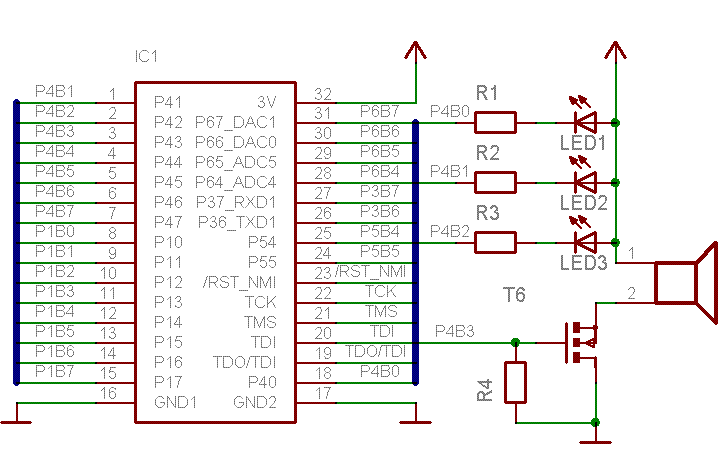
\includegraphics[width=\textwidth]{img/mikrocontrollerUNDled.png}
\caption{\em \small Schaltplan mit LEDs und Lautsprecher}
\end{figure}

\paragraph{} Die in der Aufgabenstellung gegebenen Befehle und 
ihre Wirkung sind in der folgenden Tabelle beschreiben:

\begin{longtable}{p{0.4\textwidth}p{0.5\textwidth}}

\textbf{Befehl} &
\textbf{Wirkung}
\endhead
\hline

\begin{lstlisting} 
#define LEDRT (0x01)
\end{lstlisting} &
Definition eines Präcompilermakros LEDRT.\\
\hline

\begin{lstlisting} 
P4DIR = 0x00; 
\end{lstlisting} &
Setzen der Ausgaberichtung des Portes 4 auf ausgehend.\\
\hline

\begin{lstlisting} 
a = 10;
\end{lstlisting} &
Die Variable a wird auf den dezimal Wert 10 gesetzt.\\
\hline

\begin{lstlisting} 
P4OUT = a;
\end{lstlisting} &
Schreibzugriff auf das Ausgaberegister des Ports 4. Es wird 00001010 
geschrieben, so dass das 2 und 4 Bit auf Spannung die anderen auf Ground
liegen.\\
\hline

\begin{lstlisting} 
P4OUT = 0x01; 
\end{lstlisting}  &
Erneuter Schreibzugriff auf Port 4 (genauer gesagt auf das 
Ausgaberegister).\\
\hline 

\begin{lstlisting} 
P4DIR = 0x0F;
\end{lstlisting}  &
In das Dir-Register des Portes 4 wird 11111111 geschrieben, so dass
alle Bits als Ausgabe benutzt wird. \\
\hline

\begin{lstlisting} 
a = P4IN & 0x0F;
\end{lstlisting}  &
Der Wert der am Port 4 wird mit 0x0F bitweise verundet und in a 
geschrieben. Das heißt dass die ersten 4 Bits in a genauso gesetzt 
sind wie in PIN, die anderen 4 Bits sind 0.\\
\hline 

\begin{lstlisting} 
P4OUT &= 0x08;
\end{lstlisting}  &
In das Ausgaberegister des Portes 4 wird das 4 Bit auf 1 gesetzt, falls
das Bit vorher schon 1 war, der Rest auf 0.\\
\hline 

\begin{lstlisting} 
P4OUT |= 0x01;
\end{lstlisting} &
Im Ausgaberegister des Portes 4 wird das erste Bit auf 1 gesetzt, der 
Rest beibehalten in dem das Register bitweise mit 00000001 verodert 
wird.\\
\hline

\begin{lstlisting} 
P4OUT |= LEDRT;
\end{lstlisting}  &
Unter Verwendung eines Präcompiler-Makros wird in P4OUT das erste Bit 
auf 1 gesetzt, und damit die angeschlossene LED ausschaltet.\\
\hline 

\begin{lstlisting} 
P4OUT &= ~LEDRT;
\end{lstlisting} &
Das erste Bit in P4OUT wird auf 0 gesetzt, und somit die angeschlossene
LED eingeschaltet.\\
\hline

\begin{lstlisting} 
P4OUT ^= LEDRT;
\end{lstlisting}  &
Durch ein bitweises XOR wird das erste Bit in P4OUT getoggelt. Das 
heißt wenn das Bit vorher auf 0 war ist es nun 1 und umgekehrt. \\
\hline 

\end{longtable}

Wir schalten die an Port 4 angeschlossenen LEDs an oder aus in dem wir in das Register {\em P4OUT} an die entsprechende Stelle (2-0) eine 1 oder eine 0 schreiben. 
Zuvor müssen die Portleitung auf Ausgabe (1) gesetzt werden, in dem im Register {\em P4DIR} die entsprechenden Stellen 0 gesetzt werden. Da die bereits durch die Initialsierung des Controllers passiert, müssen wir dies nicht explizit vor nehmen.
\paragraph*{}
Wir arbeiten mit Masken und logischen Operatoren. Um ein Bit ein einem Byte zum verändern, nutzen wir eine Maske die an der betreffenden Stelle eine 1 und sonst auschlielich 0 aufweist. Um ein Bit zu setzen, verodern wir die Maske bitweise mit den Register, in dem das zu modifizierende Byte steht. Um ein Bit zurück zusetzen, negieren wir die Maske und verunden sie bitweise mit dem Register. Für das toggeln eines Bits wenden wir die  Maske mit einem xor auf das Bit an. 

\lstinputlisting[caption=aufgabe1.c]{src/aufgabe1.c}


\section*{Aufgabe 2}

Wir ein Schalter geschlossen oder ein Taster gedrückt so liegt an der entsprechenden Port Leitung eine Spannung von 3 Volt gegen über GND an. Dieser Wert kann im entsprechenden Regsiter als 1 (high) aus gelesen werden.
\paragraph*{}
Um einen Wert auf einer Portleitung auszulesen, muss im DIR-Regsiter des jeweilgen Ports das entsprechende Bit auf 0 gesetzt werden. Anschließend kann der anliegende Wert (high oder low) im IN-Register des Ports ermittelt werden. Für die Aufgabe nutzen wir den Port 1, und dem entsprechend auch die Register {\em P1IN} und {\em P1DIR}.
\paragraph{}
Auch hier nutzen wir eine Maske um die für ins nicht relevanten Bits zu ignorieren. Wir lesen das gesamte Byte auf dem {\em P1IN} Register und verunden es mit einer Maske die an den relevanten Stellen 1 ist.
\paragraph{} Die in der Aufgabenstellung gegebenen Befehle und 
ihre Wirkung sind in der folgenden Tabelle beschreiben:

\begin{longtable}{p{0.4\textwidth}p{0.5\textwidth}}

\textbf{Befehl} &
\textbf{Wirkung}
\endhead
\hline

\begin{lstlisting} 
#define TasterA (0x01)
\end{lstlisting} &
Definition eines Präcompilermakros TasterA.\\
\hline

\begin{lstlisting} 
P1DIR = 0xF8;
\end{lstlisting} &
Setzen der Ausgaberichtung ersten 5 Leitungen des Ports 1 auf eingehend.\\
\hline

\begin{lstlisting} 
a = 10;
\end{lstlisting} &
Die Variable a wird auf den dezimal Wert 10 gesetzt.\\
\hline

\begin{lstlisting} 
P1OUT = a; 
/* was passiert, 
   wenn der Taster 
   an der Portleitung 
   P1.0 gedrueckt wird?
*/
\end{lstlisting} &
Es wird 00001010 ins Ausgaberegister geschreiben, an der Portleitung 3 liegt nun high an, die Portleitung 1 ist auf eingehend, daher gibt es keine Veränderungen. Durch den Druck des Tasters wird das niederwertigste Bit ebenfalls auf 1 gesetzt.\\
\hline

\begin{lstlisting} 
a = P1IN & 0x00; 
//Taste an P1.0 gedrueckt
\end{lstlisting}  &
Die Maske 0x00 überschreibt den Inhalt aus P1IN a enthält 0x00\\
\hline 

\begin{lstlisting} 
a = P1IN & 0x03; 
//Taste an P1.0 gedrueckt
\end{lstlisting}  &
Durch drücken des Tasters wird P1IN auf 00000001 gesetzt, so dass a=1 gilt. Die Verundung führt dazu das nur die 2 niederwertigsten Bits betrachtet werden.\\
\hline

\begin{lstlisting} 
a = P1IN & 0x02; 
//Taste an P1.0 gedrueckt
\end{lstlisting}  &
Durch drücken des Tasters wird P1IN auf 00000001 gesetzt, Die Verundung führt dazu das nur das zweit niederwertigste Bit betrachtet wird, so dass a=0 gilt.\\
\hline 

\begin{lstlisting} 
a = P1IN & 0x01; 
//Taste an P1.1 gedrueckt
\end{lstlisting}  &
Durch drücken des Tasters wird P1IN auf 00000010 gesetzt, Die Verundung führt dazu das nur das niederwertigste Bit betrachtet wird, so dass a=0 gilt.\\
\hline 

\begin{lstlisting} 
a = P1IN & 0x03; 
//Tasten P1.0 und 
//P1.1 gedrueckt
\end{lstlisting} &
Durch drücken des Tasters wird P1IN auf 00000011 gesetzt, Die Verundung führt dazu das nur das beide Eingabebits betrachtet werden, so dass a=3 gilt.\\
\hline

\begin{lstlisting} 
P4OUT = P1IN & TasterA; 
//Taster an P1.0
//nicht gedrueckt
\end{lstlisting}  &
Das Register P1IN enthält 00001000 nach dem Anwenden der Maske TasterA enthält P4OUT den Wert 00000000.\\
\hline 

\begin{lstlisting} 
P4OUT = P1IN & TasterA; 
//Taster P1.0 gedrueckt
\end{lstlisting} &
Das Register P1IN enthält 00001001 nach dem Anwenden der Maske TasterA enthält P4OUT den Wert 00000001.\\
\hline
\end{longtable}

\lstinputlisting[caption=aufgabe2.c]{src/aufgabe2.c}

\section*{Aufgabe 3}
\lstinputlisting[caption=aufgabe3.c]{src/aufgabe3.c}

\section*{Aufgabe 4}

Als Schalterprellen versteht man eine Veränderung des Schalterstatus während dieser eigentlich gedrückt ist. Es entsteht meist aus dem mechansichen oder elektrischen Aufbau eines Schlaters. Um das Prellen des Schalters abzufangen warten wir kurz, bevor wir erneut das Eingaberegister des Ports aus lesen. Wir versuchen dabei so lange zu warten, bis der Benutzer seine Hand vom Taster entfernt.

\lstinputlisting[caption=aufgabe4.c]{src/aufgabe4.c}
